\section{Results / Numerical Benchmarking}
\label{sec:results}

here we'll "benchmark" (aka numerically compute the cost - number of qubits and gates - of creating a lobe block-encoding) for some systems

%ideas of systems to benchmark on:
%
%- Fermi-Hubbard 
%
%- Something with just bosons
%
%- Something with fermions, antifermions, and bosons

\subsection{Pair Production/Annihilation}
\subsubsection{Hamiltonian}
In quantum field theory, particles can spontaneously be created or annihilated (hence why second quantization is useful). A particle-antiparticle pair can annihilate each other and produce a new particle, or another particle can decay and produce a particle-antiparticle pair. This can be shown in \emph{Feynman diagrams}:

\begin{figure}[h]
    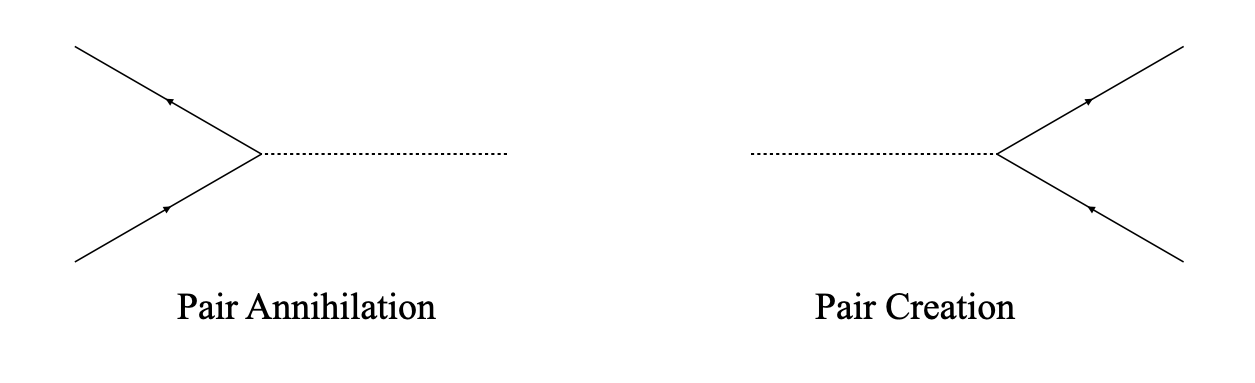
\includegraphics[width = 0.7\linewidth]{figures/creation_annihilate.png}
    \caption{Feynman diagrams corresponding to equation \ref{H_pair}}
\end{figure}


We can contrive a toy Hamiltonian that describes this procedure:

\begin{equation}
    \label{H_pair}
    H = \sum_n^{I} b_n^\dagger b_n + \sum_n^{I} d_n^\dagger d_n + \sum_n^{I} a_n^\dagger a_n + g\sum_{i,j,k}^{I} \left(b_i^\dagger d_j^\dagger a_k + b_i d_j a_k^\dagger \right).
\end{equation}

The first three terms are the kinetic energies of the individual particles ($b_n$ corresponds to a fermion, $d_n$ corresponds to an antifermion, $a_n$ corresponds to a boson). The last term describes the pair creation and pair annihilation respectively. Note that $g$ is a scalar coupling constant that describes the strength of coupling between the fermions and bosons. 
The two free parameters that control the size of the problem are $I$, the mode cutoff, and $\Omega$, the bosonic occupancy cutoff. 
\gus{Add 4 plots:}
 \begin{enumerate}
    \item gate count (3 separate lines for l/r elbows and arb. rots) USP \& ASP vs. I 
    \item gate count (3 separate lines for l/r elbows and arb. rots) USP \& ASP vs. $\Omega$
    \item n. qubits USP \& ASP vs. I
    \item n. qubits USP \& ASP vs. $\Omega$
\end{enumerate}


%\begin{figure}[h]
%    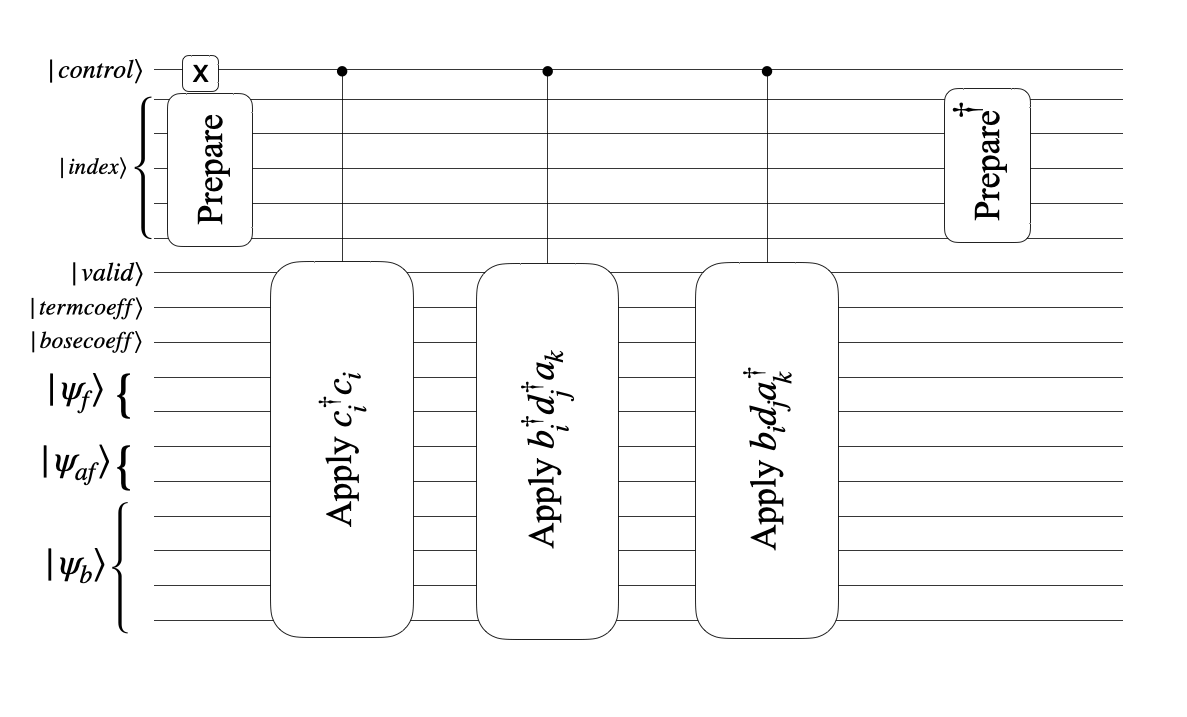
\includegraphics[width = \linewidth]{figures/H_example_LOBE_circuit.png}
%    \caption{Circuit to block encode the Hamiltonian in equation \ref{H_pair}. \gus{Need to add multiplexor control over indices}}
%\end{figure}

%In what follows, we show the explicit form of the first \textit{apply} unitary, as well as one example term from each of the following two \textit{apply} unitaries:

%\begin{figure}[h]
%    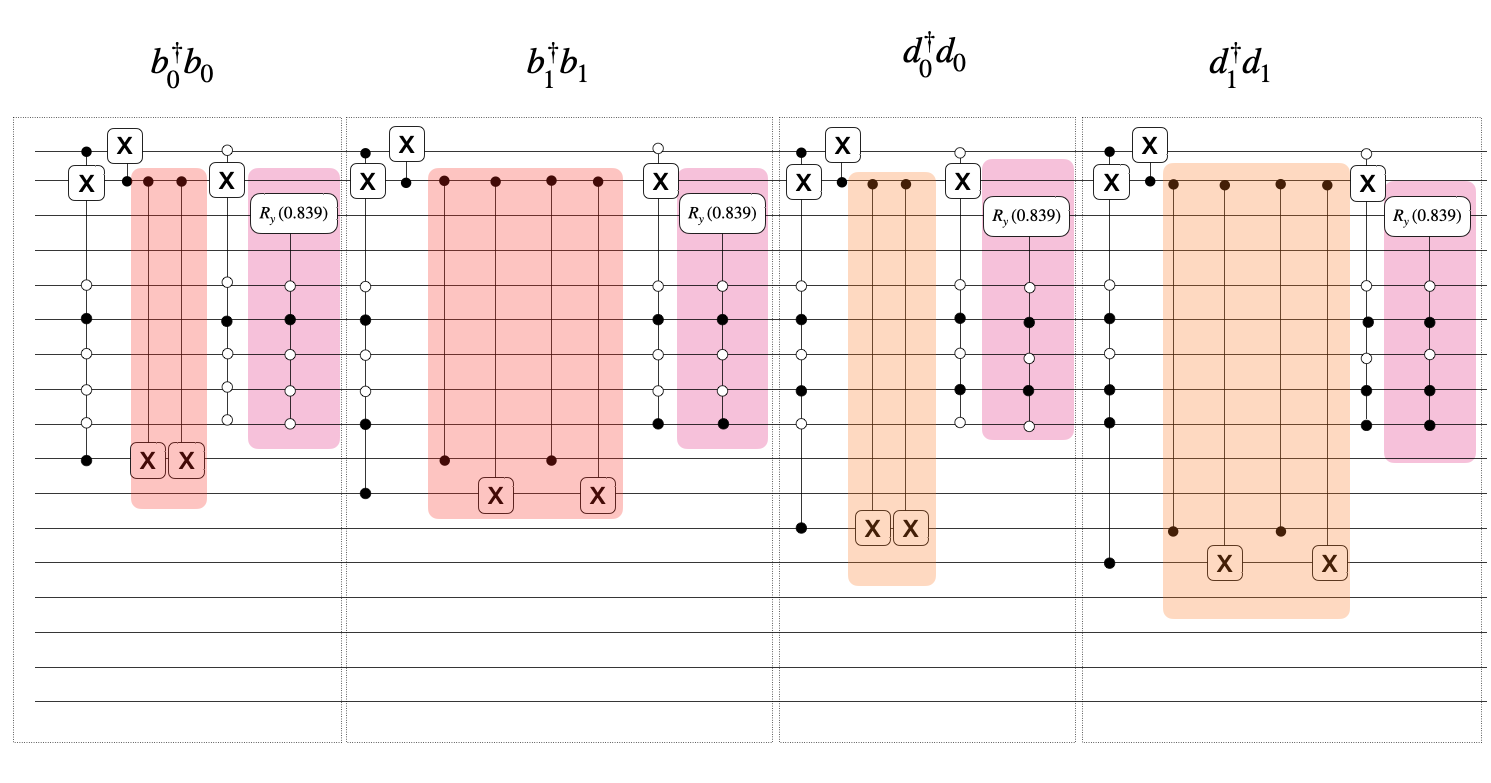
\includegraphics[width = 8cm]{figures/fermi_free.png}
%    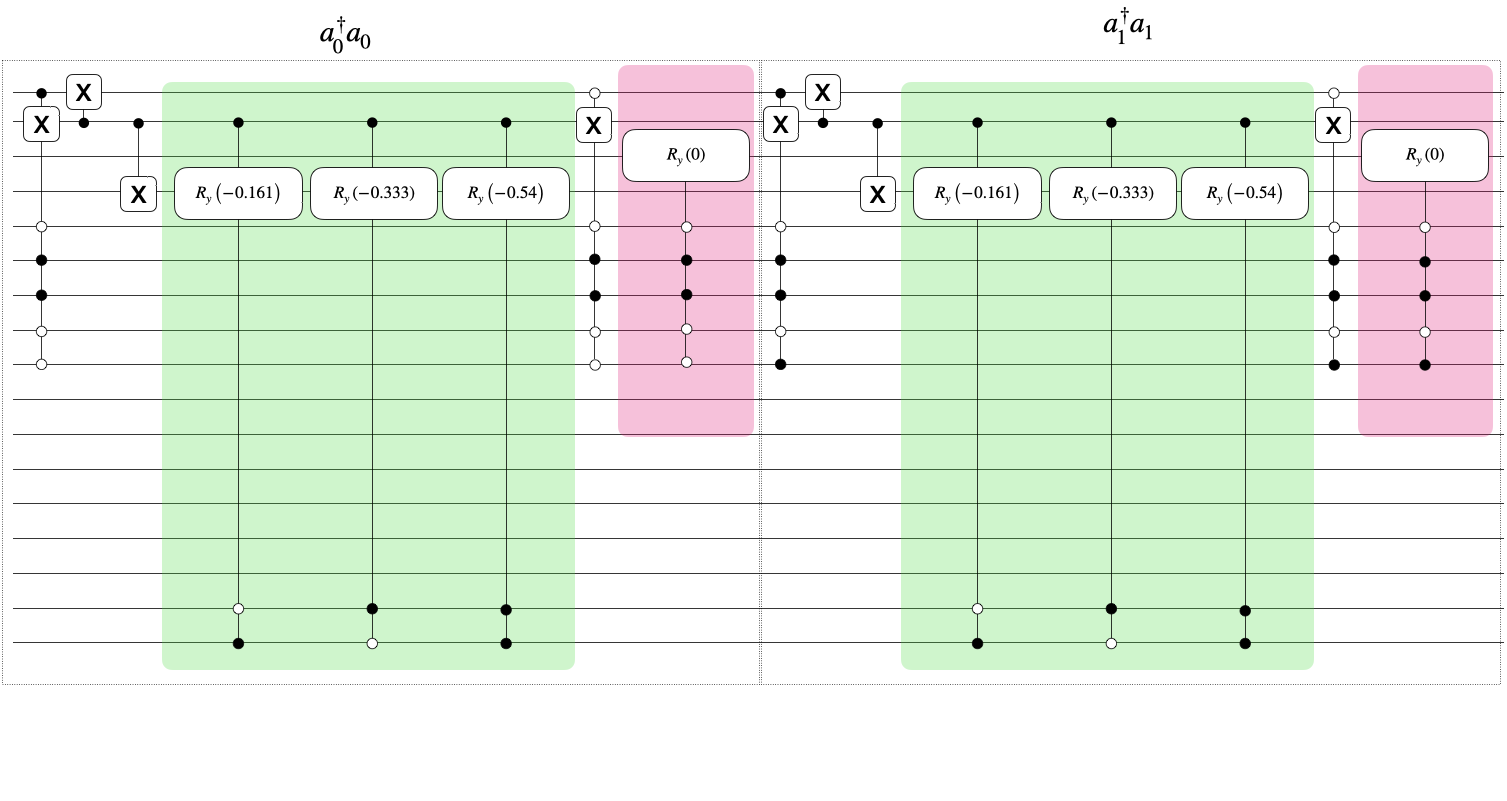
\includegraphics[width = 8cm]{figures/bose_free.png}
%    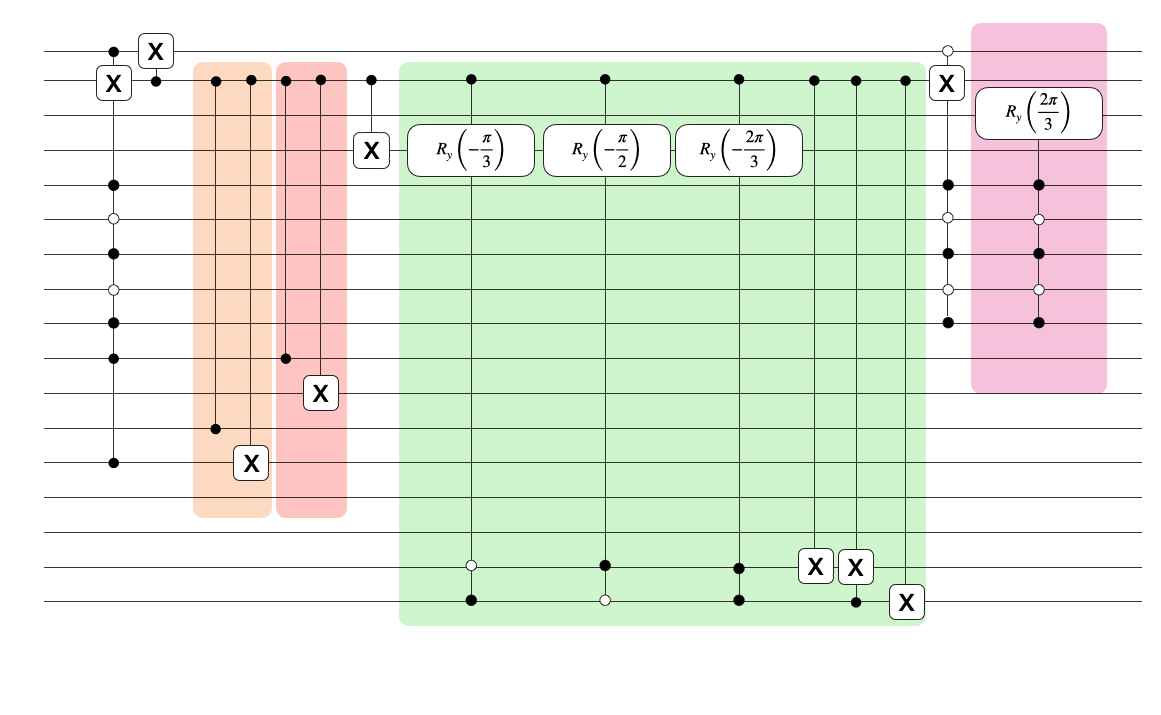
\includegraphics[width = 8cm]{figures/pair_create.png}
%    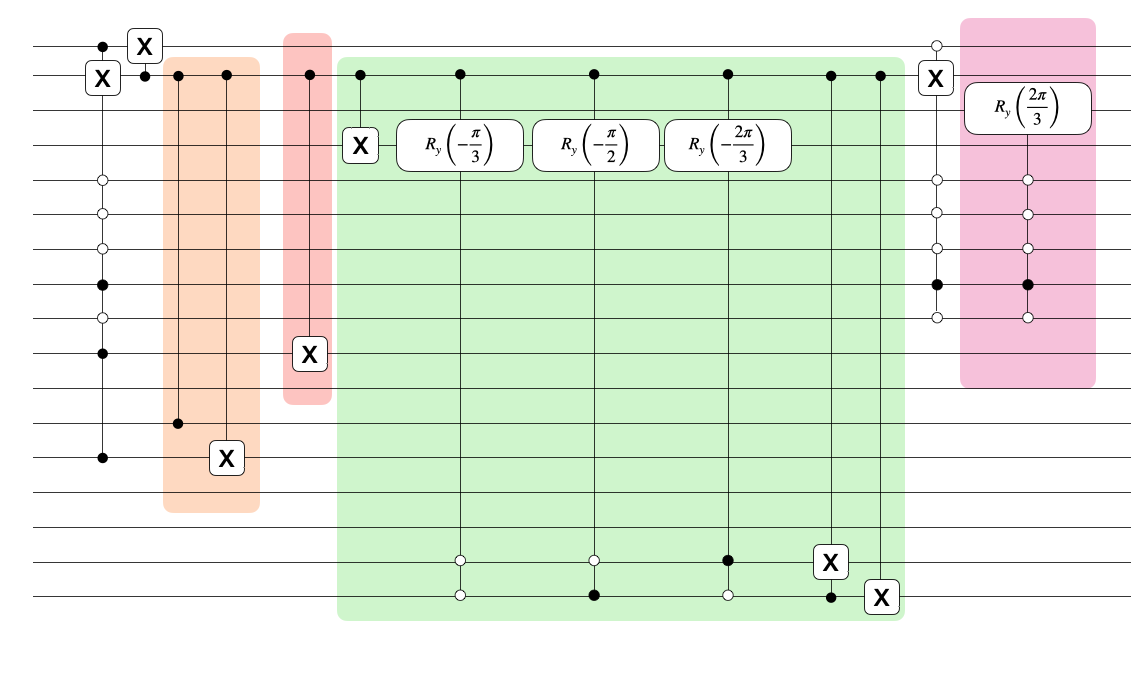
\includegraphics[width = 8cm]{figures/pair_annihilate.png}
%    \caption{Block-encoding equation \ref{H_pair}}
%\end{figure}
